\documentclass[12pt,a4paper]{scrartcl}

\usepackage[utf8]{inputenc}
\usepackage[T1]{fontenc}
\usepackage{ucs}

\usepackage[french]{babel,varioref}

\usepackage{multicol}
\usepackage{subfig}

\usepackage{enumitem}

\usepackage{color}
\usepackage{hyperref}
\hypersetup{
    colorlinks,
    citecolor=black,
    filecolor=black,
    linkcolor=black,
    urlcolor=black
}

\usepackage{amsthm}

\usepackage{tcolorbox}
\tcbuselibrary{listingsutf8}

\usepackage{ifplatform}

\usepackage{xstring}

\usepackage{fancyvrb}
% MISC

\tcbset{%
	sharp corners,%
	left=1mm, right=1mm,%
	bottom=1mm, top=1mm,%
	colupper=red!75!blue%
}

\setlength{\parindent}{0cm}

\theoremstyle{definition}
\newtheorem*{remark}{Remarque}

\usepackage[raggedright]{titlesec}

\titleformat{\paragraph}[hang]{\normalfont\normalsize\bfseries}{\theparagraph}{1em}{}
\titlespacing*{\paragraph}{0pt}{3.25ex plus 1ex minus .2ex}{0.5em}


\makeatletter
    \newcommand\resetallcnt{
    	\setcounter{lyxam@counter@topic}{0}
    	\setcounter{lyxam@counter@exercise}{0}
    	\setcounter{lyxam@counter@problem}{0}
    	\setcounter{lyxam@counter@bonus}{0}
    	\setcounter{lyxam@counter@subpart}{0}
    }
\makeatother

% Technical IDs

\newwrite\tempfile

\immediate\openout\tempfile=x-\jobname.macros-x.txt

\AtEndDocument{\immediate\closeout\tempfile}


\newcommand\IDconstant[1]{%
    \immediate\write\tempfile{constant@#1}%
}


\makeatletter
\newcommand\IDmacro{\@ifstar{\@IDmacroStar}{\@IDmacroNoStar}}

\newcommand\@IDmacroNoStar[3]{%
    \texttt{%
    	\textbackslash#1%
    	\IfStrEq{#2}{0}{}{%
    		\,\,[#2 Option%
			\IfStrEq{#2}{1}{}{s}]%
		}%
	    \IfStrEq{#3}{}{}{%
    		\,\,(#3 Argument%
			\IfStrEq{#3}{1}{}{s})%
		}
   	}
    \immediate\write\tempfile{macro@#1@#2@#3}%
}

\newcommand\@IDmacroStar[2]{%
    \@IDmacroNoStar{#1}{0}{#2}%
}


\newcommand\IDenv{\@ifstar{\@IDenvStar}{\@IDenvNoStar}}

\newcommand\@IDenvNoStar[3]{%
    \texttt{%
    	\textbackslash#1%
    	\IfStrEq{#2}{0}{}{%
    		\,\,[#2 Option%
			\IfStrEq{#2}{1}{}{s}]%
		}%
	    \IfStrEq{#3}{}{}{%
    		\,\,(#3 Argument%
			\IfStrEq{#3}{1}{}{s})%
		}
   	}
    \immediate\write\tempfile{env@#1@#2@#3}%
}

\newcommand\@IDenvStar[2]{%
    \@IDenvNoStar{#1}{0}{#2}%
}


\newcommand\@IDoptarg{\@ifstar{\@IDoptargStar}{\@IDoptargNoStar}}

\newcommand\@IDoptargStar[2]{%
	\vspace{0.5em}
	--- \texttt{#1%
		\IfStrEq{#2}{}{:}{\,#2:}%
	}%
}

\newcommand\@IDoptargNoStar[2]{%
	\IfStrEq{#2}{}{%
		\@IDoptargStar{#1}{}%
	}{%
		\@IDoptargStar{#1}{\##2}%
	}%
}


\newcommand\IDkey[1]{%
	\@IDoptarg*{Option}{{\itshape "#1"}}%
}


\newcommand\IDoption[1]{%
	\@IDoptarg{Option}{#1}%
}


\newcommand\IDarg[1]{%
	\@IDoptarg{Argument}{#1}%
}
\makeatother

\usepackage[fr]{lyxam}


\begin{document}

\renewcommand\labelitemi{\raisebox{0.125em}{\tiny\textbullet}}
\renewcommand{\labelitemii}{---}

\title{%
	Le package \texttt{lyxam}:\\%
	des mises en forme clés en main\\%
	pour des fiches d'exercices\\%
	{\footnotesize Code source disponible sur \url{https://github.com/bc-latex/ly-xam}.}\\%
	{\footnotesize Version \texttt{0.3.0-beta} développée et testée sur \macosxname{}.}%
}
\author{Christophe BAL}
\date{2017-12-02}

\maketitle


\vspace{2em}

\hrule

\tableofcontents

\vspace{1.5em}

\hrule

\newpage



\section{Introduction}

Le but du tout petit package \verb+lyxam+ est de fournir un moyen simple de rédiger des feuilles d'exercices pour des entraînements ou des évaluations dans le cadre d'un enseignement.




\section{Les options du package}

Avant d'entrer dans le vif du sujet, nous donnons ici toutes les options utilisables lors de l'appel du package via \verb+\usepackage[...]{lyxam}+.

\begin{itemize}
	\item \verb+en+, valeur par défaut
	\footnote{
		Sorry for the french frogs that we are... (Trad. : Désolé pour les grenouilles françaises que nous sommes...)
	}, et \verb+fr+ permettent d'indiquer d'utiliser l'anglais ou le français pour tous les textes ajoutés par \verb+lyxam+.

	\item \verb+hf+, valeur par défaut, et \verb+nohf+ demandent d'afficher ou non les en-têtes et les pieds de page.
	Les lettres \verb+hf+ sont pour "\textbf{h}-eaders" et "\textbf{f}-ooters", soit "en-tête" et "pied de page" en français.

	\item \verb+pts+, valeur par défaut, et \verb+nopts+ servent à voir ou non les points donnés pour chaque exercice.

	\item \verb+noshort+, valeur par défaut, et \verb+short+ demandent d'utiliser le nom long ou abrégé, si possible, pour indiquer les types d'exercices, les points et le temps.

	\item \verb+src+, valeur par défaut, et \verb+nosrc+ feront afficher ou non les sources utilisées.

	\item \verb+about+, valeur par défaut, et \verb+noabout+ feront afficher ou non les informations complémentaires sur les thèmes, les exercices et les parties.

	\item Voici les différents styles de mise en forme disponibles (dans le dossier \verb+examples+ se trouvent divers \verb+PDFs+ donnant un aperçu de ces styles prédéfinis).
	\begin{itemize}[label={\small\textbullet}]
        \item Style par défaut, \verb+mini+ propose une mise forme minimaliste utilisant le moins de fioritures possibles.
        
        \item \verb+apmep+ est inspiré fortement de la mise en forme des sujets de BAC que l'on trouvait en 2017 sur le site \href{https://www.apmep.fr}{APMEP} (Association des Professeurs de Mathématiques de l'Enseignement Public).
        
        \item \verb+book+ fournit une mise forme utile dans un livre ou un cours. Attention car cette option ne crée pas d'en-têtes, pas de pieds de page, et elle ne mettra pas en forme de capsules pour le nom et le prénom des élèves même si cela est demandé.
        
        \item \verb+ecolo+ mélange les styles \verb+mini+ et \verb+book+ pour produire des devoirs très peu consommateur d'espaces.
        
        \item \verb+linebox+ utilise des lignes et des cadres (il a été conçu à l'origine pour les corrigés de l'auteur de \verb+lyxam+).

\end{itemize}
\end{itemize}


\begin{remark}
	Dans la suite de cette documentation nous invoquons juste l'option \verb+fr+.
	Autrement dit, nous passons par \verb+\usepackage[fr]{lyxam}+ donc ce sera le style par défaut \verb+mini+ qui donnera la mise en forme.
\end{remark}




\section{Quel devoir donnez-vous ?}

    \subsection{La commande \texttt{\textbackslash exam}}

La commande \verb+\exam+ permet de donner des informations générales à propos du devoir.
Le code ci-dessous utilise toutes les options disponibles, et la figure \ref{style:default} \vpageref{style:default} donne un aperçu du rendu obtenu dans ce cas.

\begin{tcblisting}{listing only}
\exam[deliver  = short,%
      kind     = D.S.,%
      nb       = 1,%
      subnb    = Sujet A,%
      subject  = Mathématiques,%
      theme    = Probabilités,%
      sector   = Série Scientifique,%
      class    = 1S4,%
      location = Lycée MONGE (Chambéry),%
      date     = 20/10/2017,%
      time     = 2h]
\end{tcblisting}


\begin{figure}[!tbp]
  \setlength{\fboxrule}{1.5pt}
  \centering
  \fbox{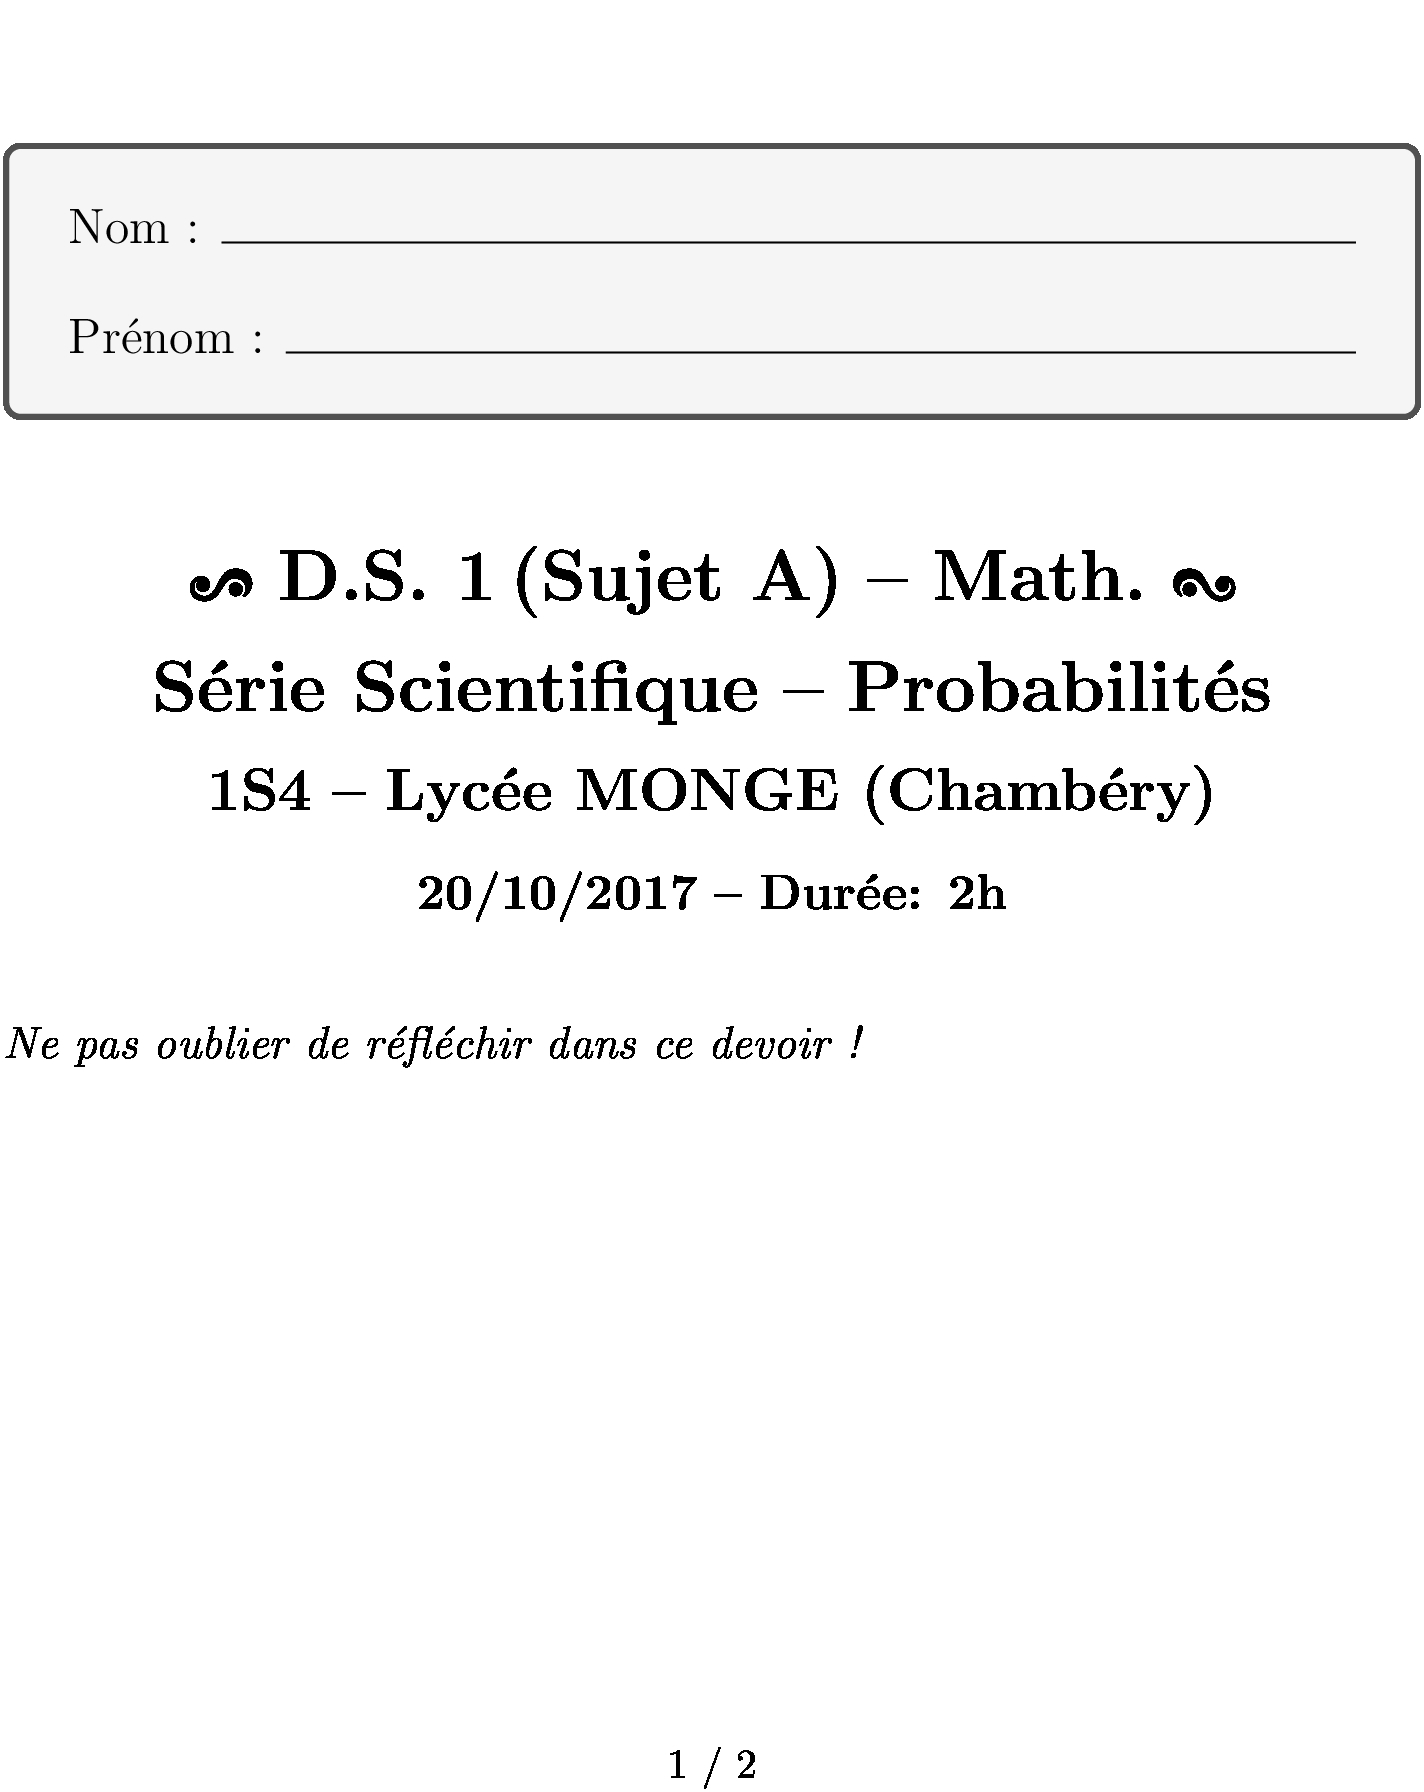
\includegraphics[width=0.43\linewidth]{example-doc[fr]-0.jpg}}
  \hfill
  \fbox{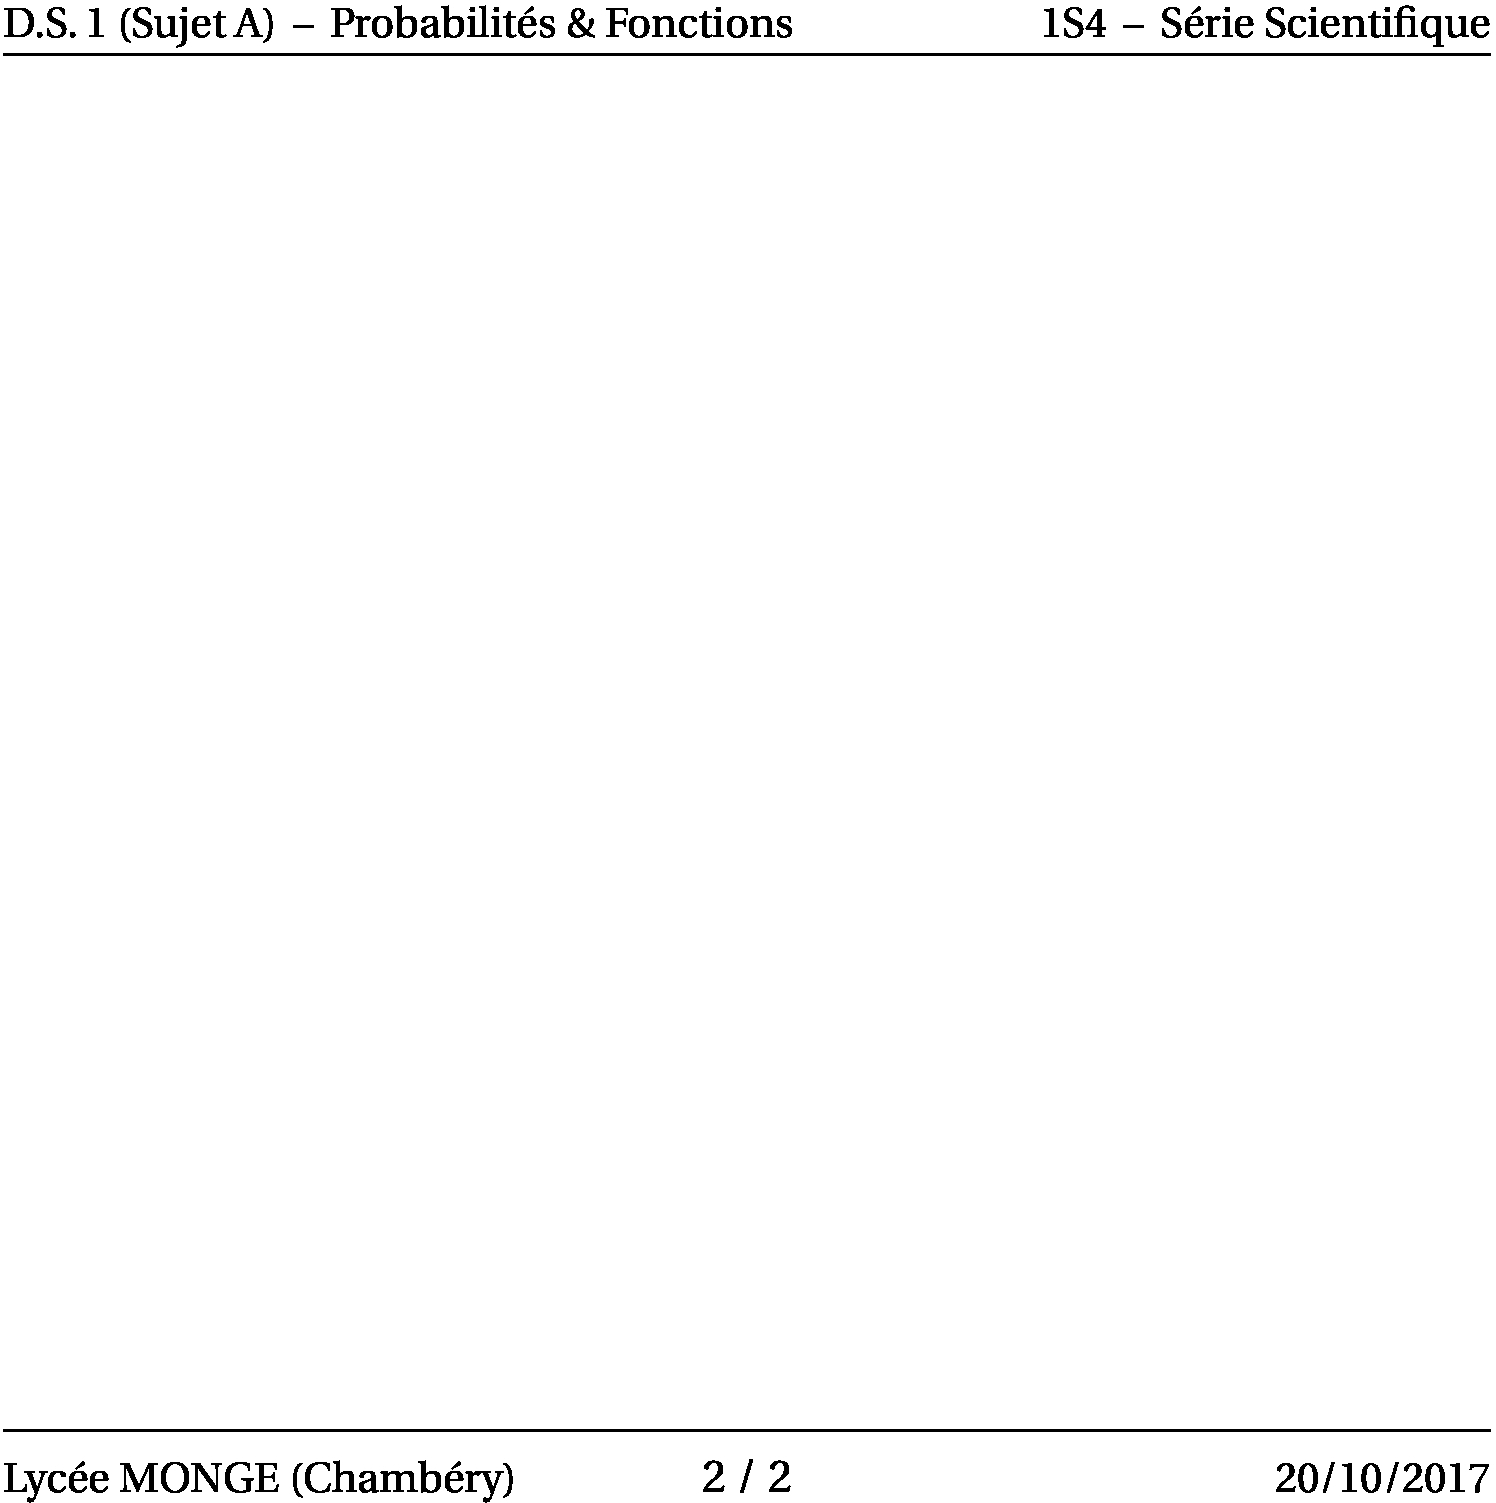
\includegraphics[width=0.43\linewidth]{example-doc[fr]-1.jpg}}
  \caption{Style par défaut.}
  \label{style:default}
\end{figure}

Expliquons maintenant en détail le rôle de chacun des paramètres qui sont tous optionnels. Lorsqu'aucune valeur par défaut n'est indiquée, c'est que cette valeur est un texte vide.

\begin{enumerate}
    \item \verb+deliver+, valant \verb+no+ par défaut, est pour un sujet à rendre avec la copie.
    \begin{itemize}
        \setlength\itemsep{0em}

        \item On peut indiquer \verb+deliver = short+ où \emph{"short"} signifie \emph{"court"}. Ceci affichera une "petite" capsule où l'étudiant renseignera son prénom et son nom. Idéal pour le format \verb+A4+.

        \item Avec \verb+deliver = long+, la capsule sera plus grande. Idéal pour le format \verb+A5+.

        \item Ne pas utiliser l'option revient à passer par \verb+deliver = no+.
    \end{itemize}

    \item \verb+kind+, valant \verb+Test+ par défaut, est le type de devoir : un \emph{"D.S."}, un \emph{"D.M."}, une \emph{"Interrogation Surprise"}, une \emph{"Fiche d'entraînement"}, une \emph{"Activité"}...
    Vous noterez que le terme \emph{"devoir"} ne se limite pas juste aux devoirs notés.

    \item \verb+nb+ est le numéro du devoir.

    \item \verb+subnb+ permet d'indiquer une sorte de numérotation secondaire. C'est utile par exemple pour indiquer \emph{"Sujet A"}, \emph{"Sujet B"} ...

    \item \verb+subject+ permet de donner la thématique générale du devoir comme par exemple \emph{"Mathématiques"}, \emph{"Informatique Générale"}...

    \item \verb+theme+ complète la thématique générale en indiquant un ou des points particuliers comme par exemple \emph{"Probabilités"}, \emph{"Réseaux"} ...

    \item \verb+sector+ sert à indiquer une section, au sens administratif, à laquelle s'adresse le devoir. Par exemple, pour un sujet de Baccalauréat S en France, on serait amené à utiliser \verb+sector = Série Scientifique+.

    \item \verb+class+ indique la classe et/ou le groupe auquel est destiné le devoir.

    \item \verb+location+ vous permet d'indiquer un lieu géographique, typiquement un établissement scolaire ou universitaire.

    \item \verb+date+ est pour la date du devoir.

    \item \verb+time+ est pour la durée du devoir.
\end{enumerate}


    \subsection{Fiche technique}

\IDmacro{exam}{11}{}

\IDkey{kind} le type de devoir, la valeur par défaut étant \verb+Test+.

\IDkey{deliver} pour un sujet à rendre, ou non, avec une zone pour le nom et le prénom de l'étudiant. Trois valeurs possibles : \verb+no+, valeur par défaut, \verb+long+ et \verb+short+.

\IDkey{nb} le numéro du devoir.

\IDkey{subnb} une numérotation secondaire du devoir.

\IDkey{subject} la matière, le sujet au sens large du devoir.

\IDkey{theme} un sous-thème ou une sous-partie de la matière ou du sujet du devoir.

\IDkey{sector} un secteur, une section, au sens administratif, à laquelle s'adresse le devoir.

\IDkey{class} la classe concernée par le devoir.

\IDkey{location} le lieu géographique où a lieu le devoir.

\IDkey{date} le texte donnant la date du devoir.

\IDkey{time} le texte indiquant juste la durée du devoir.




\newcommand\exosoptions{
\IDkey{pts} le nombre de points avec le cas particulier de $0$ qui demande d'afficher "Non noté".

\IDkey{time} la durée de l'exercice.

\IDkey{id} un texte de votre choix pour remplacer le numéro (ceci a pour effet de bloquer temporairement la numérotation).

\IDkey{title} un titre.

\IDkey{about} une petite indication liée à l'exercice (comme par exemple qu'il ne s'adresse qu'aux élèves motivés).

\IDkey{src} la source utilisée pour confectionner l'exercice.
}


\section{Indiquer vos exercices}

    \subsection{Important pour la suite}

Rappelons que tous les exemples utilisés dans cette documentation ont été obtenus en utilisant \verb+\usepackage[fr]{lyxam}+ dans le préambule ce qui charge le style par défaut parmi les différents styles proposés (voir le dossier \verb+examples+ pour choisir un style prédéfini).


    \subsection{Différents types d'exercices}

Voici l'ensemble des commandes disponibles pour indiquer un type d'exercice.

% All kind of level 2 contexts - START
\begin{itemize}
\makeatletter
    \item \verb+\activity+ correspond à "\lyxam@text@activity{}".
    
    \item \verb+\bonus+ correspond à "\lyxam@text@bonus{}".
    
    \item \verb+\exercise+ correspond à "\lyxam@text@exercise{}".
    
    \item \verb+\mcq+ correspond à "\lyxam@text@mcq{}".
    
    \item \verb+\praticalwork+ correspond à "\lyxam@text@praticalwork{}".
    
    \item \verb+\problem+ correspond à "\lyxam@text@problem{}".
\makeatother
\end{itemize}
% All kind of level 2 contexts - END

Dans la suite, nous donnerons des exemples principalement avec la commande \verb+\exercise+. Ceci n'est pas gênant car le principe reste identique pour les autres commandes.


    \subsection{Numérotation minimaliste}

En \textbf{compilant deux fois} au moins, \verb+lyxam+ va pouvoir donner une numérotation minimaliste de vos exercices. Tout d'abord, ci-dessous on obtient classiquement des exercices tous numérotés où vous noterez que chaque type d'exercice admet sa propre numérotation.


\begin{tcblisting}{}
\exercise
\exercise
\problem
\problem
\end{tcblisting}


Que souhaite-t-on avoir dans un sujet ne contenant qu'un seul problème et un seul bonus ? Nul besoin ici d'avoir un numéro pour ces derniers. C'est ce que fait \verb+lyxam+.

\resetallcnt{}

\begin{tcblisting}{}
\exercise
\exercise
\problem
\bonus
\end{tcblisting}



    \subsection{Indiquer le barème}

La commande \verb+\exercise+ dispose de plusieurs options dont l'une permet de donner le nombre de points attribués à un exercice où lorsque l'on indique $0$ point le package indique une exercice non noté (voir la section suivante pour un exemple). Voici comment donner un barème.

\resetallcnt{}

\begin{tcblisting}{}
\exercise[pts = 5]
Bla, bla, bla, bla, bla, ...
\end{tcblisting}


    \subsection{Cacher le texte "Exercice"}

La version étoilée \verb+\exercise*+ permet de cacher le contexte qui du point de vue de \verb+lyxam+ sera ici le texte "Exercice". Ceci est surtout pratique pour les sous-parties présentées un peu plus bas. Dans ce genre de situation, il faut obligatoirement donner un titre.

\begin{tcblisting}{}
\exercise*[title = Juste mon titre]

Bla, bla, bla, bla, bla, ...
\end{tcblisting}


    \subsection{Toutes les options en action}

Les fiches techniques données un peu plus bas expliquent le champs d'utilisation de chaque option.
\textit{\textbf{Attention !} L'environnement} \verb+tcblisting+ \textit{utilisé dans ce document ne montre pas ci-dessous la note de bas page numérotée $\lceil$a$\rfloor$ qui donne la source utilisée.}

\begin{tcblisting}{}
\exercise[pts   = 0,
          time  = 3 jours,
          id    = facultatif,
          title = Devinette,
          about = Pour spécialiste uniquement,
          src   = Le livre des experts]
Bla, bla, bla, bla, bla, ...
\end{tcblisting}


    \subsection{Fiches techniques}

Toutes les options données ci-dessous sont facultatives.

\bigskip


% IDmacro - All kind of level 2 contexts - START
\IDmacro{activity}{6}{}

\IDmacro{bonus}{6}{}

\IDmacro{exercise}{6}{}

\IDmacro{mcq}{6}{}

\IDmacro{praticalwork}{6}{}

\IDmacro{problem}{6}{}
% IDmacro - All kind of level 2 contexts - END

\exosoptions{}



\section{Indiquer des sous-parties dans vos exercices}

    \subsection{Un exemple suffit\dots{} ou presque}

La commande \verb+\subpart+, avec les mêmes options que les commandes de type \verb+\exercice+, sert pour des sous-parties d'un exercice qui seront numérotées relativement aux exercices comme le montre l'exemple suivant.

\resetallcnt{}

\begin{tcblisting}{}
\exercise
\subpart
\subpart

\exercise
\subpart
\subpart
\end{tcblisting}


    \subsection{Fiche technique}

Toutes les options données ci-dessous sont facultatives et identiques à celles vues précédemment.

\bigskip


% IDmacro - All kind of level 3 contexts - START
\IDmacro{subpart}{6}{}
% IDmacro - All kind of level 3 contexts - END

\exosoptions{}



\section{Regrouper vos exercices par thèmes}

    \subsection{Un exemple suffit\dots{} ou presque}

La commande \verb+\topic+, avec les mêmes options que les commandes de type \verb+\exercice+, sert juste à regrouper des exercices par thématiques : fût un temps où dans les brevets du collège, il y avait une partie numérique et une autre géométrique.
Chaque nouvelle utilisation de \verb+\topic+ remet juste à zéro la numérotation des sous-parties mais pas celles des contextes de type \verb+\exercice+.

\resetallcnt{}

\begin{tcblisting}{}
\topic
\exercise
\exercise

\topic
\exercise
\end{tcblisting}


    \subsection{Fiche technique}

Toutes les options données ci-dessous sont facultatives et identiques à celles vues précédemment.

\bigskip


% IDmacro - All kind of level 1 contexts - START
\IDmacro{topic}{6}{}
% IDmacro - All kind of level 1 contexts - END

\exosoptions{}



\section{Personnaliser les numérotations}

    \subsection{Un petit exemple}

En mettant un peu les mains dans le cambouis, on peut modifier à sa guise la numérotation de chaque type d'exercice. Voici un exemple tapé directement dans un fichier \verb+tex+, ce qui impose d'employer \verb+\makeatletter...\makeatother+.

\resetallcnt{}

\begin{tcblisting}{}
\makeatletter
    \renewcommand\lyxam@counter@exercise@style[1]{-- \arabic{#1} --}
\makeatother

\exercise
\exercise
\end{tcblisting}


    \subsection{Fiches techniques}

% IDmacro - All styles for counters - START
\IDmacro{lyxam@counter@activity@style}{0}{1}

\IDmacro{lyxam@counter@bonus@style}{0}{1}

\IDmacro{lyxam@counter@exercise@style}{0}{1}

\IDmacro{lyxam@counter@mcq@style}{0}{1}

\IDmacro{lyxam@counter@praticalwork@style}{0}{1}

\IDmacro{lyxam@counter@problem@style}{0}{1}

\IDmacro{lyxam@counter@subpart@style}{0}{1}

\IDmacro{lyxam@counter@topic@style}{0}{1}
% IDmacro - All styles for counters - END

\IDarg{} the \LaTeX{} counter associated to the context.


\section{Utiliser un préambule}

    \subsection{Un exemple avec toutes les options}

L'environnement \verb+\preamble+ sert à rédiger un ou plusieurs paragraphes en préambule de tout un examen, d'un thème, d'un exercice ou d'une partie.
Il propose deux options : l'une \verb+center+ pour centrer le contenu à l'intérieur du préambule, l'autre \verb+scale = ...+ un coefficient multiplicatif pour la largeur allouée au préambule (ce coefficient est multiplié à \verb+\linewidth+ pour calculer la largeur souhaitée).

\resetallcnt{}

\begin{tcblisting}{}
\begin{preamble}[scale = 0.75, center]
    Cet exercice est indépendant \verb+;-)+. Bla, bla, bla, bla, bla, bla,
    bla, bla, bla, bla, bla, bla, bla, bla, bla, bla, bla, bla, bla,\dots
\end{preamble}

\exercise

\begin{preamble}
    Dans cet exercice, tout trace de recherche sera prise en compte à
    condition de ne pas explorer le Pôle Nord quand on s'intéresse
    au Pôle Sud. Quoique...
\end{preamble}

Trouver ....
\end{tcblisting}


    \subsection{Fiches techniques}

\IDenv{preamble}{2}{}

\IDkey{scale} un nombre, valant $1$ par défaut, qui sera multiplié à la largeur d'une ligne pour obtenir la largeur souhaitée pour le préambule.

\IDkey{center} un booléen, valant \verb+false+ par défaut, pour centrer ou non le contenu du préambule (notez que \verb+center+ est un raccourci de \verb+center = true+).





\section{Historique}

Tous les changements sont décrits en anglais uniquement dans le dossier \verb+change_log+ : voir le code source de \verb+lyxam+ sur \verb+github+. Nous ne donnons ici qu'un très bref historique de \verb+lyxam+.

\begin{description}[leftmargin=1em]
    \setlength\itemsep{1em}

    \item[2017-12-02] Nouvelle version mineure \verb+0.3.0-beta+ du package.
    \begin{itemize}
        \item L'option de package \verb+mini+ fournit un style de mise en forme minimaliste. Ce sera le style par défaut.

        \item L'option de package \verb+book+ a été ajouté pour insérer dans un document de type cours ou livre.

        \item L'option de package \verb+ecolo+ mélange les mises en forme de \verb+mini+ et \verb+book+ pour rédiger des devoirs en utilisant le moins d'espaces possible.        
    \end{itemize}

    \item[2017-11-28] Nouvelle version mineure \verb+0.2.0-beta+ du package.
    \begin{itemize}
        \item L'option de package \verb+linebox+ fournit un nouveau style de mise en forme.

        \item Les options de package \verb+short+ et \verb+noshort+ permettent d'indiquer ou non en abrégé, si possible, les types d'exercices, les points et le temps.

        \item Les options de package \verb+about+, valeur par défaut, et \verb+noabout+ feront afficher ou non les informations complémentaires sur les thèmes, les exercices et les parties.

        \item L'option \verb+render+ de la macro \verb+\exam+ a été renommée \verb+deliver+ (ce qui semble plus correct).

        \item Ajout de deux options à l'environnement \verb+\preamble+ : l'une pour centrer ou non le contenu, et l'autre pour choisir la largeur occupée par le préambule.

        \item Il est maintenant possible de personnaliser la numérotation des exercices.
    \end{itemize}

    \item[2017-11-12] Nouvelle version mineure \verb+0.1.0-beta+ du package.
    \begin{itemize}
        \item Les nouvelles options \verb+hf+ et \verb+nohf+ permettent au chargement du package de montrer ou cacher les en-têtes et les pieds de page.

        \item L'option \verb+preamble+ de la macro \verb+\exam+ disparait pour laisser place au nouvel environnement \verb+\begin{preamble}...\end{preamble}+ utilisable n'importe où.

        \item Pour la macro \verb+\exam+, tous les paramètres sont optionnels.

        \item Pour les macros du type \verb+\exercise+, le paramètre \verb+note+ a été renommé \verb+about+.

        \item En interne, l'utilisation de \verb+simplekv+ a permis une refonte complète du code en simplifiant la méthode à utiliser pour créer de nouvelles mises en page "maison".
    \end{itemize}

    \item[2017-11-03] Première version publique \verb+0.0.0-beta+ du package.
\end{description}



\end{document}
